\subsection{Adaptación del análisis espectral a señales reales con una frecuencia de muestreo dada}

Para hacer nuestros análisis espectrales
numéricos de una señal $x \in \IR^{n}$, hemos
usado la dimensión $n$ de la señal en cuestión 
para buscar, en base a máximos globales
del espectro 
$\Sigma_{x}: [0, \frac{n}{2}] \longrightarrow [0,1]$, la
mejor frecuencia $\omega$ para aproximar la gráfica
de $x$ en base a un sinusoide discreto
de dimensión $n$. \\

Note que en esta discusión nunca hablamos de 
parámetros importantes para, de forma canónica, hacer
un análisis espectral, como lo son la
duración en tiempo de la señal o la frecuencia
de muestreo.

\begin{defi}
\label{def: tiempo y frec de muestreo}
La cantidad de muestras tomadas (de forma uniforme)
de una señal por unidad de tiempo 
será denotada por $F_{s}$ y llamada \textbf{frecuencia
de muestreo} de la señal. A la cantidad de unidades de
tiempo que dura la medición se le denotará por $T$. 
A la cantidad total de muestras tomadas se le denotará
por $L$.
\end{defi}
Observe que, para poder dividir una unidad
de tiempo en $F_{s}$ subintervalos de igual longitud,
se deben divider al eje del tiempo con los puntos
\begin{equation}
t_{k} := t_{0} + h k, \hspace{0.2cm}
\textit{con } h := \frac{1}{F_{s}}.
\end{equation}
A tal constante $h$, definida como el recíproco de la frecuencia
de muestreo, se le llama el \textbf{paso temporal} de la señal. \\

De las definiciones se sigue de inmediato que
\begin{equation}
\label{eq: relacion L, T Fs}
L = T F_{s}.
\end{equation}
\begin{figure}[H]
	\sidecaption{
	Adoptamos la convención de empezar a medir 
	un bloque de $F_{s}$ mediciones desde que inicia la
	unidad de tiempo (que, en el caso de la figura, se ha
	fijado como segundos).
	\label{fig: Fs 1}
	}
	\centering
	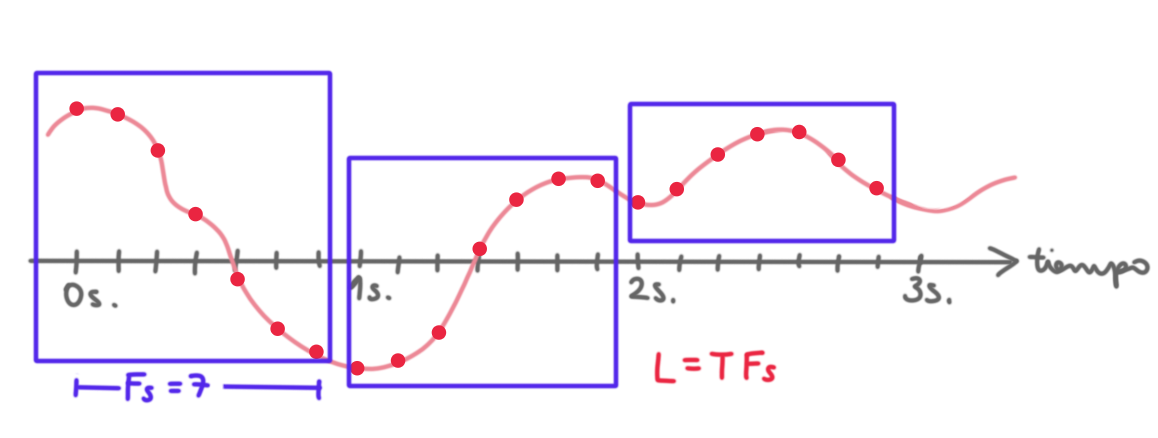
\includegraphics[scale = 1]{Fs_1} 
\end{figure}	

Nosotros, por el momento, sólo nos
hemos enfocado en buscar
una frecuencia $\omega \in [0, \frac{n}{2}]$ que de lugar
a un sinusoide que aproxime bien la gráfica
de $x$;
observe que, al hacer esto, hemos supuesto de forma
implícita que estamos estudiando una señal
de duración una unidad de tiempo
(i.e. $T = 1$) y de longitud $n$
(i.e. $L = F_{s} = n$). \\
Supongamos ahora que
tenemos una señal $x$ que consta de $L$ mediciones, siendo
$F_{s}$ la frecuencia de muestreo.
\begin{figure}[H]
	\sidecaption{
	Para la imagen, hemos fijado $F_{s}= 10$
	y $L = 40$.
	\label{fig: frecuencia 1}
	}
	\centering
	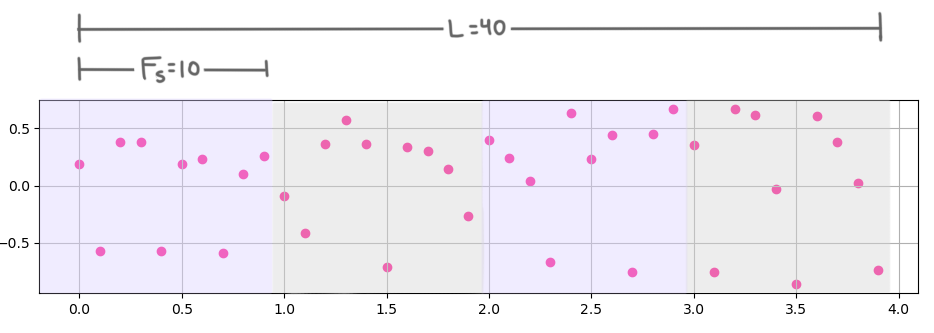
\includegraphics[scale = 0.45]{frecuencia_1} 
\end{figure}	

Sea ahora $2 \leq n \leq L$ y
supogamos que
se hizo el análisis
espectral 
de una sección $x_{|n}$ de tal señal
que conste de $n$ puntos
(usando el espectro
$\Sigma_{x}: [0, \frac{n}{2}]
\longrightarrow [0,1]$).
Digamos que, como conclusión de ese análisis, se
obtuvo que un sinusoide de frecuencia $\omega \in [0, \frac{n}{2}]$
ajusta bien \textit{esa sección particular 
$x_{|n}$
de la señal $x$}.
\begin{figure}[H]
	\sidecaption{
	Para la imagen, hemos fijado $n= 6$;
	se calculó que la mejor frecuencia para ajustar 
	los primeros $6$ puntos que componen la señal
	original $x$ es $w = 2$.
	\label{fig: frecuencia 2}
	}
	\centering
	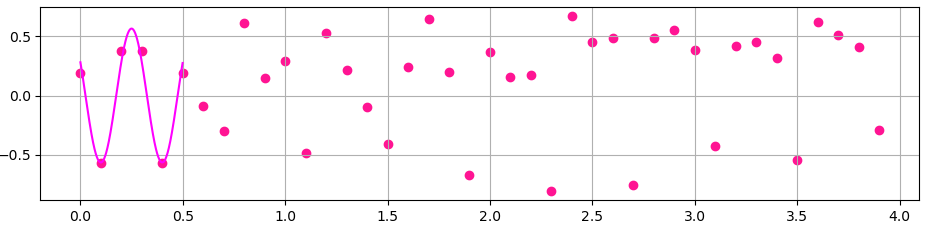
\includegraphics[scale = 0.45]{frecuencia_2} 
\end{figure}	

Observe que, en general, si se quisiera usar
directamente una frecuencia de $w$ para ajustar
a la señal $x$, la aproximación lograda en los
$n$ puntos escogidos previamente puede no ser válida.
\begin{figure}[H]
	\sidecaption{
	Usando los datos de la figura \ref{fig: frecuencia 2}, podriamos
	intentar en un principio usar a un sinusoide de frecuencia $2$
	para intentar modelar a la señal, pero un sinusoide de tal frecuencia,
	como es el caso de esta figura, puede que ni siquiera sea adecuado
	para modelar el pedazo $x_{|n}$ original a partir del cual se obtuvo
	la frecuencia $\omega$.
	\label{fig: frecuencia 2}
	}
	\centering
	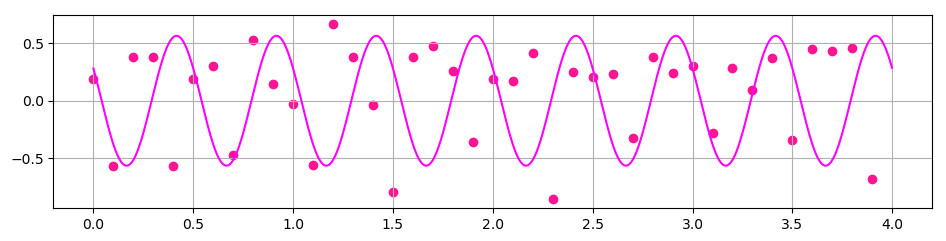
\includegraphics[scale = 0.45]{frecuencia_3} 
\end{figure}
Esto se debe a que	
tal frecuencia $\omega$ es buena para aproximar
a dichos $n$ puntos cuando se ha tomado como
unidad de tiempo a $n$, pero, 
por la forma en que fue muestreada la señal original $x$,
son $F_{s}$ (y no necesariamente $n$) la cantidad de puntos
que conforman una unidad. Así, puesto que con $\omega$
ciclos de un sinusoide se aproximaron $n$ puntos, 
la frecuencia que debe escogerse para aproximar a todos los $L$
puntos es
\begin{equation}
\label{eq: rel frecuencia real y ficticia}
\tilde{w} := \frac{F_{s}}{n} \omega.
\end{equation}

\begin{figure}[H]
	\sidecaption{
	Es con una simple regla de tres que se deduce
	la relación \eqref{eq: rel frecuencia real y ficticia}.
	\label{fig: frecuencia real}
	}
	\centering
	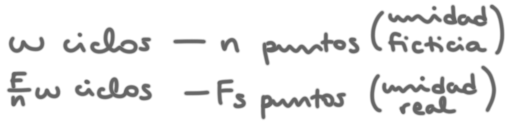
\includegraphics[scale = 1.4]{frecuencia_real} 
\end{figure}	
\begin{figure}[H]
	\sidecaption{
	Según los datos de las figuras
	\ref{fig: frecuencia 1}
	y \ref{fig: frecuencia 2}, con un sinusoide de frecuencia
	$\tilde{\omega} = 10/3$ se aproximan bien a los seis
	puntos en base a los cuales se encontró a la primera
	frecuencia $\omega$.
	\label{fig: frecuencia 4}
	}
	\centering
	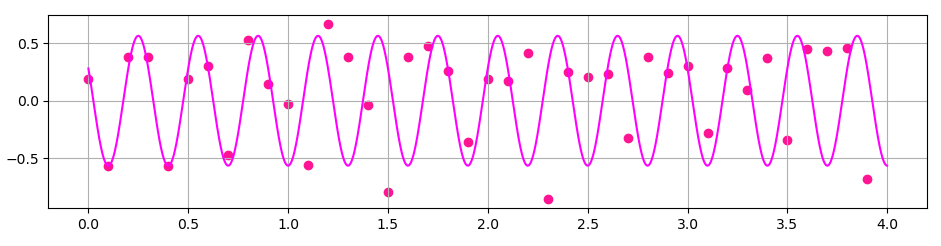
\includegraphics[scale = 0.45]{frecuencia_4} 
\end{figure}